
\documentclass[journal]{IEEEtran}

% *** CITATION PACKAGES ***
\usepackage[style=ieee]{biblatex} 
\bibliography{example_bib.bib}    %your file created using JabRef
\usepackage {graphicx}
% *** MATH PACKAGES ***
\usepackage{amsmath}

% *** PDF, URL AND HYPERLINK PACKAGES ***
\usepackage{url}
% correct bad hyphenation here
\hyphenation{op-tical net-works semi-conduc-tor}
\usepackage{graphicx}  %needed to include png, eps figures
\usepackage{float}  % used to fix location of images i.e.\begin{figure}[H]
\usepackage{amssymb}
\usepackage{inputenc}
\usepackage[thinc]{esdiff}

\begin{document}
% paper title
\title{Delay-dependent Robust Stability Analysis of Power Systems with PID Controller}

% author names 
\author{ Authors: Eashwar Sathyamurthy  Akwasi A Obeng}
        
% The report headers
\markboth{ENPM667 Controls of Robotics Systems. Technical Report 9, November 2019}
{Shell \MakeLowercase{\textit{et al.}}: Bare Demo of IEEEtran.cls for IEEE Journals}

% make the title area
\maketitle

% As a general rule, do not put math, special symbols or citations
% in the abstract or keywords.
\begin{abstract}
  This technical report examines the robust stability of a power system, which is based on proportional-integral-derivative load
frequency control and involves uncertain parameters and time delays. This report examines a power system model which  is transformed into a closed-loop system with feedback control. The purpose of this report is to verify new augmented Lyapunov-Krasovskii (LK)
functional to employ the new Bessel-Legendre inequality. The new Bessel-Legendre inequality is used to estimate the derivative of the functional to obtain
a maximum lower bound. This report also verifies and provides a detailed description of stability criterion of the power system obtained by employing the LK functional and Bessel-Legendre inequality. Finally,
this report validates the proposed method by applying it to practical numerical examples.
\end{abstract}

\begin{IEEEkeywords}
  Index Terms - To be modified later
\end{IEEEkeywords}

\section{Introduction}
% Here we have the typical use of a "W" for an initial drop letter
% and "RITE" in caps to complete the first word.
% You must have at least 2 lines in the paragraph with the drop letter
% (should never be an issue)

\IEEEPARstart{W}{ith} the growing population, the demand for efficient power systems have increased drastically. Efficient power systems have the characteristics of high stability margin and less time delays. These characteristics are attainable if the operating frequency of the power system fluctuate within a small range of equilibrium value and the load frequency control (LFC) can control these fluctuations. During the process of data transmission, there is always a possiblity of occurance if time delays. These time delays occur randomly which makes it impossible to predict.  Therefore, gaining insights on robust stability of power systems with time delays and uncertain parameters can help to overcome this problem. \\

The most research methods employed in time-delay systems are based on the Lyapunov direct time-domain method. Through the construction of the Lyapunov-Krasovskii (LK) functional, the stability of the system is analyzed with the aid of the Lyapunov stability theory, after which the stability criterion is derived. Finally, the stability margin of the system is obtained by employing the linear matrix inequality (LMI) toolbox.This report aims to improve the upper bound of the time delay of the system by proposing an augmented LK functional and using the Bessel-Legendre inequality to estimate the derivative of the functional. This study assumes that the forward channel of the controller possesses time delays and the inertia time constant of both the prime mover and speed governor may have uncertain parameters in the system. A time-varying delay power system model is established with uncertain parameters based on proportional-integral-derivative (PID) load frequency control. An appropriate LK functional is constructed, and the robust stability of the system is then analyzed using the Lyapunov stability theory. Finally, the robust stability criterion of the system is obtained by employing the Bessel-Legendre inequality discussed in Ref. [9], and the stability margin that the system can withstand is solved using an LMI toolbox. The advantages and effectiveness of the proposed method are demonstrated by comparing the results of the proposed method with those of previous methods under the two controller gains.\\

The variables used in this study are defined as follows:
 $R^n$ and $R^{n*m}$ denote n-dimensional vectors and $n * m$ dimensional matrices in the real number domain, respectively; $R^T$ and $R^-1$ represent the transpose and inverse of a matrix, respectively; I and 0 are identity and zero matrices, respectively;  P  should be greater than 0 means that the matrix P is symmetric and positive; $Sym{X}=X+X^T$; ‘*’ represents symmetric terms in a symmetric matrix; and diag(···) denotes a diagonal matrix. \\


\section{Concepts Needed}

\subsection{Legendre Polynomials}
A brief overview of Legendre polynomials obtained by solving Legendre
ODE is provided below. \\ 

Legendre ODE is given as follows
 \begin{equation}
  (1-x^2)\diff[2]{f}{x} - 2x\diff{f}{x} + k(k+1)y = 0 \\
\end{equation} \\

Solution to ODE is obtained as follows:

Step 1: Convert Equation to the form shown below
\begin{equation}
\diff[2]{f}{x} + p(x)\diff{y}{x}  + q(x)y = G(x)
\end{equation}

Therefore we have,
\begin{equation}
     \diff[2]{f}{x} - \frac{2x}{1-x^2}\diff{f}{x} + \frac{k(k+1)}{1-x^2}y = 0
\end{equation}


Step 2: Use power series solution about $x_0 = 0$\\
Therefore, 
\begin{align}
  Y(x) &= \sum_{n=0}{\infty}a_nx^n  \\
  Y'(x) &= \sum_{\infty}{n=0}na_nx^{n-1} \\
  Y''(x) &= \sum_{n=0}^{\infty}n(n-1)a_nx^(n-2)
 \end{align}
 
 Plug this back into the ODE to get the recurrence relation
 below
 \begin{equation}
a_{n+2} = \frac{(n-k)(n+k+1)}{(n+2)(n+1)}
\end{equation}

Solving recurrence relation\\

Odd Index solution
\begin{align}
    a_3 &= \frac{a_1(1-k)(2+k)}{3!} \\
    a_5 &= \frac{a_1(k-3)(k-1)(k+2)(k+4)}{5!} \\
\end{align}

Polynomial Soln for k(even or odd)

Set $a_k$ to calculate $a_{k-2},a_{k-4}$
\begin{equation}
a_n = \frac{(n-k)(n+k+1)}{(n+2)(n+1)} a_n 
\end{equation}
replace n by k-2
\begin{align}
  a_{k-2k}&= \frac{-1(k)(k-1)}{2(2k-1)} \\
  a_k &= \frac{-1(2k-2)!}{2^k(k-1)!(k-2)!}
\end{align}
Similarly,
\begin{equation}
a_{k-4} = \frac{(-1)^2(2k-4)!}{2(2^k)(k-2)!(k-4)!}
\end{equation}
    Therefore the general formula

    \begin{equation}
    a_{k-2m} = \frac{-1^m(2k-m)!}{(m!)(2^k)(k-m)!(k-2m)!}
  \end{equation}


  
    Therefore
    \begin{equation}
    P_k(x) = \sum_{m=0}^{k/2} 
  \end{equation}

   Properties \\
    Legendre Polynomials are orthogonal
    \begin{align}
      %ie int_-1^1 P_{k_1}P_{k_2} &= 0 %for k_1 neq k_2
    (2n-1)xP_(n-1)(x) = nP(x) + (n-1)P_(n-2)(s) n = 2, 3 ...
  \end{align}

    

%\begin{equation}
  %(1-x^2)
%\end{equation}
\subsection{Bessle Legendre Inequalities}
 \begin{align}
   \int_{-h}^{0}x(u)Rx(u)du \geq \frac{1}{h}
   \begin{bmatrix}
     \omega_0 \\
     . \\
     . \\
     . \\
     \omega_n
   \end{bmatrix}
   R_N
   \begin{bmatrix}
  \omega_0 \\
  . \\
  . \\
  . \\
  \omega_n
\end{bmatrix}
 \end{align}

 where R is symmetric positive definite matrix
 and 
 \begin{align}
   R_N &= diag(R,3R,...,(2N+1)R) \\
   \omega_k&= \int_{-h}^{0}P_k(u)x(u)du, 
 \end{align}
 for all natural numbers k and x is a square integrable function
 from an open interval,I to $R^n$
\subsection{Lyapunov-Krasovskii Functional}
\subsection{Prime mover}
\subsection{Speed governor}
\section{Controllability and Stability Analysis}
\subsection{Controllability} The above linear time variant power system is controllable only if the matrix \\
\begin{equation}
\begin{bmatrix}
B & AB & AB^2 
\end{bmatrix}
\text{preserves rank}
\end{equation}

where $t_{0}$ is the initial time \\
$t_{f}$ is the final time
Checking the condition for controllability: \\
We have \\

\begin{equation}
B =
\begin{bmatrix}
0 \\
 0 \\
 \frac{1}{T_{G}}
\end{bmatrix}
A =
\begin{bmatrix}
\frac{D}{M} & \frac{D}{M} & 0 \\
 0 & \frac{-1}{T_{T}} & \frac{1}{T_{T}}\\
 \frac{-1}{T_{G}R} & 0 & \frac{-1}{T_{G}} \\
\end{bmatrix} \\
\end{equation}
\newline
\begin{equation}
AB =
\begin{bmatrix}
0 \\
 \frac{1}{T_{G}T_{T}} \\
 \frac{1}{T_{G}^2}
\end{bmatrix}
A^2B =
\begin{bmatrix}
\frac{D}{MT_{G}T_{T}} \\ \\
 \frac{T_{G} + T_{T}}{T_{G}^2T_{T}^2} \\ \\
 \frac{1}{T_{G}^2}
\end{bmatrix}
\end{equation}
\\
\begin{equation}
\begin{bmatrix}
B & AB & AB^2 
\end{bmatrix}
= 
\begin{bmatrix}
0 &  0 & \frac{D}{MT_{G}T_{T}} \\ \\
0 & \frac{1}{T_{G}T_{T}} & \frac{T_{G} + T_{T}}{T_{G}^2T_{T}^2} \\ \\
 \frac{1}{T_{G}}  & \frac{1}{T_{G}^2} &  \frac{1}{T_{G}^2}
\end{bmatrix}
\end{equation}
\\
\begin{equation}
\text{det}
\begin{bmatrix}
B & AB & AB^2 
\end{bmatrix}
= \frac{-D}{MT_{G}^3T_{T}^2} \neq 0
\end{equation}
Therefore the the matrix $[B \quad AB \quad A^2B]$ preserves rank. Hence, the power system is controllable which simultaneously implies that the system is stabilizable.

\section{System Model and Derivations}

\begin{figure}
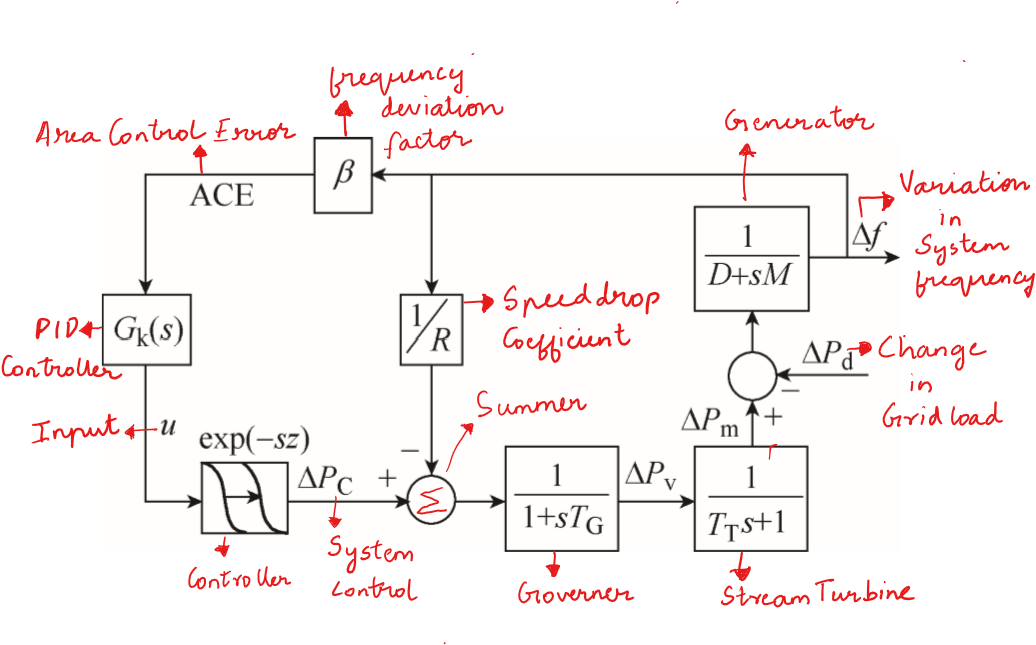
\includegraphics[width=\linewidth]{systemmodel.png}
  \caption{System}
  \label{fig:System1}
\end{figure}


The system above controls the frequency of the load(LFC) to some desired output. \\

Whenever there is a change in grid load, the system adjust the frequency for the new load by 
doing the following.

\begin{enumerate} 
  \item Generator generates a new frequency 
  \item Frequency deviation factor($\beta$) is used to get the error
  \item Error is fed into PID to handle frequency variation
  \item A control signal is generated to control the governor
  \item Output is fed into Governor(acts as an actuator) to control valve
  \item Valve is opened based on signal
  \item Variation in valve opening causes a desired power change  
 \end{enumerate} \\ \\
From the figure above, the equations of motion can be represented as 


\begin{align}
  \diff{\Delta f}{t} &= \frac{-D}{M}\Delta f + \frac{D}{M}\Delta P_m - \frac{1}{M}\Delta{P_d} \\ \\
  \diff{\Delta P_m}{t} &= \frac{-\Delta P_m}{T_T} + \frac{P_v}{T_T} \\ \\
  \diff{\Delta P_v}{t} &= \frac{-1}{T_GR}{\Delta f} - \frac{1}{T_G}{\Delta P_v}  \\ \\
  ACE(t) &= \Delta f \beta
\end{align} \\

This can be represented in state space equation as
\begin{align}
  \diff{x(t)}{t} &= Ax_o(t) + Bu(t- h(t)) + F(\omega{t}) \\
  y_o(t) &= Cx_o(t)
\end{align}

where
\begin{align}
  x_o(t) &= [\Delta f \quad  \Delta P_m  \quad \Delta P_v]  \\
  y_o(t) &= ACE
\end{align}

\begin{align}
  A &=
\begin{bmatrix}
  \frac{D}{M} & \frac{D}{M} & 0 \\
  0 & \frac{-1}{T_T} & \frac{1}{T_T} \\
  \frac{-1}{T_GR} & 0 & \frac{-1}{T_G}
\end{bmatrix}
\quad
  B =
\begin{bmatrix}
  0 \\
  0 \\
  \frac{1}{T_G}
\end{bmatrix}
\\ \\
  F &=
\begin{bmatrix}
  \frac{1}{M} & 0 & 0
\end{bmatrix}
\quad
  C = 
\begin{bmatrix}
  \beta & 0 & 0
\end{bmatrix}
\end{align}

\begin{equation}
w(t) = \Delta P_d \quad u(t-h(t)) = \Delta P_c(t)
\end{equation}

Meaning of Symbols
\begin{align}
  \Delta f &-> \text{Variation in system frequency}  \\
  \Delta P_m &-> \text{Variation in Mechanical Power} \\
  \Delta P_v &-> \text{Variation in Control Valve Opening} \\
  ACE(t) &-> \text{Area Controller Error} \\
  h(t) &-> \text{Delay Stability Margin} \\
  u(t-h(t)) &-> \text{Input with Delay} \\
  \Delta P_d &-> \text{Changes in Grid load} \\
  \Delta P_c &-> \text{Changes in System Control  Signals} \\
  M &-> \text{Moment of Inertia} \\
  D &-> \text{Damping Coefficient of generator} \\
  T_T &-> \text{Inertia time of the Generator of Steam Turbine} \\
  T_G &-> \text{Inertia time of the Governor of the unit } \\
  R &-> \text{Speed Drop coefficient of the Governor} \\
  \beta &-> \text{frequency Deviation Factor} 
\end{align} 

The PID Controller handles the Area Controller Error(ACE) and produces a feedback 
using the equation stated as follows

\begin{equation}
  u(t)=K_pACE(t) + K_I\int ACE(t)dt + K_D \diff{ACE(t)}{dt}
\end{equation}
where
\begin{align}
  K_I &-> \text{Integral gain}\\
  K_P &-> \text{Proportional gain} \\
K_D &->\text{Derivative gain}
\end{align}


The virtual state and output variables can be writen as follows
\begin{align}
  \bar{x}_0(t) &= 
  \begin{bmatrix}
    x_0^T(t) & \int y_0^T(t) dt
  \end{bmatrix}^T \\
  \bar{y}_0(t) &= 
  \begin{bmatrix}
    y_0^T(t) & \int y_0^T(t)dt & \diff{y_0^T(t)}{t}
  \end{bmatrix}^T
\end{align}

Because CB = 0, we have the transformation
\begin{align}
  \diff{\bar{x}}{t} &= \bar{A}\bar{x}_0(t) + \bar{B}u(t-h(t)) + \bar{F}\omega (t) \\
  \bar{y}_0(t) &= \bar{C}\bar{x}_0(t) + \bar{D}_w\omega(t) \\
  u(t)&= -K\bar{y}_0(t)
\end{align}

\begin{align}
  \diff{\bar{x}_{0}(t)}{t} = \bar{A}\bar{x}_{0}(t) + \bar{A}_{d}\bar{x}_{0}(t-h(t)) + \bar{B}_w\omega(t) \\
\end{align}
where $\bar{A}_{d}= -\bar{B}K\bar{C}$ ,$\bar{B}_w = \bar{F} - \bar{B}K\bar{D}_w $\\

Consider an equilibrium point (point for which $\diff{\bar{x}_0(t)}{t} = 0$) at $\bar{x}_0^*(t)$
Therefore,           
\begin{equation}
  0 = \bar{A}\bar{x}_0^*(t) + \bar{A}_d\bar{x}_0^*(t-h(t)) + \bar{B}_w\omega(t)
\end{equation}

Perfoming State Transformation where $x(t) = \bar{x}(t)-\bar{x}_0^*(t)$, we have
\begin{equation}
  \diff{x}{t} = \bar{A}x(t) + \bar{A}_dx(t-h(t)) \\
\end{equation}
where 
\begin{align}
  \bar{A} &=
  \begin{bmatrix}
    \frac{-D}{M} & \frac{1}{M} & 0 & 0 \\
    0 & \frac{-1}{T_T} & \frac{1}{T_T} & 0 \\
    \frac{-1}{T_GR} & 0& \frac{-1}{T_G} & 0 \\
    \beta & 0 & 0 & 0
  \end{bmatrix} \\
  \bar{A}_d &=
  \begin{bmatrix}
    0 & 0 & 0 & 0 \\
    0 & 0 & 0 & 0 \\
    \frac{\beta D K_D}{MT_G} - \frac{\beta K_{P}}{T_G} & \frac{-\beta K_D}{MT_G} & 0 & \frac{-K_1}{T_G} \\
    0 & 0 & 0 & 0
  \end{bmatrix}
\end{align}
Since the parameters of the power system experience some disturbance, this is accounted for by the following: \\
 let $\alpha$ be the disturbance deviation for prime mover \\
 let $\beta$ be the disturbance deviation for Governor \\
 
 Because the values of the deviations are extremely small, we use the percentage error.
 Therefore,the new value of $T_T$ due to error change can be accounted for as

 \begin{align}
   T_{Ta} &\epsilon [(1-\alpha \%)T_T, (1+\alpha\%)T_T] \\
   T_{Ga} &\epsilon [(1-\gamma \%)T_G, (1+\gamma\%)T_G]
 \end{align}
 \begin{align}
   T_{Ta} &-> \text{Inertia time constant for prime mover} \\
   T_{Ga} &-> \text{Inertia time contant for Governor}
 \end{align}
  Given the values above, $T_T$ can be expressed as
  \begin{align}
    T_T = \frac{1+\gamma \alpha \%}{(1-\alpha \%)(1+\alpha \%)} T_Ta
  \end{align}
  where $\gamma \epsilon [-1\quad1]$ is a constant \\ 
   
  We can however write the above equation in a more general form by letting $\gamma$ be function 
  on the same interval. Therefore we write in a more compact form as follows
 \begin{align}
   \frac{1}{T_{Ta}} = \frac{\alpha _1}{T_T} + f_1(t)\frac{\alpha _2}{T_T}\\
   \frac{1}{T_{Ga}} = \frac{\gamma _1}{T_G} + f_2(t)\frac{\gamma _2}{T_G}
\end{align}
 where 
 \begin{align}
   f_1(t),&f_2(t) \epsilon  [-1,1] \\
   \alpha _1 &= \frac{1}{(1-\alpha)(1+\alpha\%)} , \quad \alpha _2 = \alpha\% \alpha _1 \\
   \gamma _1 &= \frac{1}{(1-\gamma)(1+\gamma\%)} , \quad \gamma _2 = \gamma \%\gamma
 \end{align}

 Therefore the new equation including delay is 
\begin{align}
  \diff{x}{t}=(A_0 + \Delta A_0)x(t) + (A_d + \Delta A_d)(x(t-h(t))),
 \end{align}
 where
 \begin{flalign}
   &[\Delta A_0 \quad \Delta A_d] = HF(t)[E_1 \quad E_2] \\
   &H = I  \\
   F(t) &= diag\{0,f_1(t),f_2(t),0\} \\
   &A_0 = 
   \begin{bmatrix}
     \frac{-D}{M} &\frac{1}{M} &0 &0 \\
     0 &\frac{-\alpha _1}{T_T} &\frac{\alpha}{T_T} &0 \\
     -\frac{\gamma}{T_GR} &0 -&\frac{\gamma _1}{T_G} &0 \\
     \beta& 0 & 0 & 0
   \end{bmatrix} \\
   &A_d =
   \begin{bmatrix}
     0&0&0 &0 \\
     0 &0&0&0 \\
     \frac{\gamma _1 \beta D K_D}{MT_G} - \frac{\gamma _1\beta K_p}{T_G}&0 -&\frac{\gamma _1\beta K_D}{MT_G} &-\frac{\gamma _1 K_1}{T_G} \\
     0& 0 & 0 & 0
   \end{bmatrix} \\
   &E_1=
   \begin{bmatrix}
     0&0&0&0 \\
     0&-\frac{\alpha _2}{T_1} &{\alpha _2}{T_T} &0  \\
     -\frac{\gamma _2}{T_GR} &0 &\frac{-\gamma _2}{T_G} &0 \\
     0&0&0&0 
   \end{bmatrix} \\
   &E_2 =
   \begin{bmatrix}
     0&0&0 &0 \\
     0 &0&0&0 \\
     \frac{\gamma _2 \beta D K_D}{MT_G} - \frac{\gamma _2\beta K_p}{T_G}&0 -&\frac{\gamma _2\beta K_D}{MT_G} &-\frac{\gamma _2 K_1}{T_G} \\
     0& 0 & 0 & 0
   \end{bmatrix}
 \end{flalign}

\section{Robust Stability}


\section{Results}
%Show plots of any data collected and describe with words what your plots are showing. Describe the relationship between variables and time. Remember to number all your figures.  This is the most critical part affect the technical achievement.\\
%No picture, table, schematic, or graph should appear without a name (generally of the form Fig.1 o Table 1). %~\ref{fig:ecg} or Table~\ref{table:Exps}), 
%None should appear without a reference to them by name in the main body of the writing.
%All figures and tables must be discussed in the text, including what it is, significant observations, and analysis. \\
%Capitalize “Table” and “Fig.” any time they are accompanied by specific table or figure numbers. Examples: “The measured data are plotted in Fig. 2. The figure shows a linear relationship in....”. “The table shows …” vs. “The data of Table 3…” \\

%\begin{table}[!ht] %[H]
%\centering
%\label{table:Exps}
%\begin{tabular}{ll}
%Student &  Max Temperature \\ \hline
%aabbbccc &  $35^{\circ}$   \\
%eeeddd &   $54^{\circ}$ \\
%eeeddd &   $54^{\circ}$ \\
%\end{tabular}
%\caption{Temperature measurements performed for session 1.}
%\end{table}

%you can use a table generator from here: https://www.tablesgenerator.com/#

%Use your word processor to make “real tables” (i.e., boxed in, etc.). Center all tables and include a heading and caption with the appropriate table number below each table. For example, “Table 1: Temperature measurements performed for session 1.” 

%Figures must be centered, and the figure number and caption is centered beneath the
%figure. For example, “Figure~\ref{fig:ecg}”. 

%\begin{figure}[H]%[!ht]
%\begin {center}
%\caption{Illustrations, graphs, and photographs may fit across both columns, if necessary. Your artwork must be in place in the article.}
%\label{fig:ecg}
%\end {center}
%\end{figure}

%Always spell out table or Table. Give abbreviation of Figure, i.e., Fig., when used in
%the middle to end of sentence, but spell it out when used at the very start of the
%sentence. \\


%All graphs must be done with a computer (i.e., spreadsheet software such as
%Microsoft Excel or even Matlab.). Do not include hand drawn graphs unless
%specifically instructed to do so.  \\
%Include a leading zero when a number’s magnitude is less than 1 (use 0.83 instead of
%writing .83). \\
%Use your word processor for Greek symbols for common engineering quantities as $\beta$, $\pi$, $\gamma$ ,$\Omega$ . 

\section{Discussion and Summary}
%Discuss any interesting result related to the materials used or to any claim from the introduction. Discuss your measurements using engineering terms (accuracy, precision, resolution, etc).  Give technical conclusions. Restate the main objectives and how or to what degree they were achieved. What principles, laws and/or theory
%were validated by the experiment? Describe some applications of your results and comment any possible recommended future work.



% if have a single appendix:
%\appendix[Proof of the Zonklar Equations]
% or
%\appendix  % for no appendix heading
% do not use \section anymore after \appendix, only \section*
% is possibly needed

% use appendices with more than one appendix
% then use \section to start each appendix
% you must declare a \section before using any
% \subsection or using \label (\appendices by itself
% starts a section numbered zero.)
%


\appendices
%\section{Hand calculations (or name your title for appendix subtitle)}
%List any extra evidence such as photos of the session, that may help you support your claims.
%You can include all hand calculations, extra graphs and plots, simulation results, etc. 

 %use section* for acknowledgment
\section*{Acknowledgment}
%The authors would like to thank...



% references section

% can use a bibliography generated by BibTeX as a .bbl file
% BibTeX documentation can be easily obtained at:
% http://mirror.ctan.org/biblio/bibtex/contrib/doc/
% The IEEEtran BibTeX style support page is at:
% http://www.michaelshell.org/tex/ieeetran/bibtex/
%\bibliographystyle{IEEEtran}
% argument is your BibTeX string definitions and bibliography database(s)
%\bibliography{IEEEabrv,../bib/paper}
%
% <OR> manually copy in the resultant .bbl file
% set second argument of \begin to the number of references
% (used to reserve space for the reference number labels box)

%use following command to generate the list of cited references

\printbibliography


%Examples of references:  \\[0.001in]

%Example of data book:\\[0.1in]
%[2] National Operational Amplifiers Databook. Santa Clara: National Semiconductor
%Corporation, 1995 Edition, p. I-54. \\[0.1in]
%Example of textbook: \\[0.1in]
%[3]M. Young, The Technical Writer’s Handbook. Mill Valley, CA: University Science, 1989.\\[0.1in]
%Example of scientific journal paper:\\[0.1in]
%[4] J.W. Smith, L.S. Alans and D.K. Jones, “An operational amplifier approach to
%active cable modeling”, IEEE Transactions on Modeling, vol. 4, no. 2, 1996, pp.
%128-132.\\[0.1in]
%Example of conference paper proceedings:\\[0.1in]
%[5] J.W. Smith, L.S. Alans and D.K. Jones, “Active cable models for lossy
%transmission line circuits”, in Proc. 1995 IEEE Modeling Symposium, 1996, pp.
%1086-89.\\[0.1in]

%Example of Internet web page:\\[0.1in]
%[6] Approximate material properties in isotropic materials. Milpitas, CA: Specialty
%Engineering Associates, Inc. web site: www.ultrasonic.com, downloaded Aug. 20,
%2001. 

%List and number all bibliographical 
%references at the end of your paper in {\bf 9 or 10 point} Times, with 10-point interline spacing. When referenced within the text, enclose the citation number in square brackets, for example [1]. \\
%Use IEEE format. Cite any external work that you used (data sheets, text books, Wikipedia articles, . . . ). If you get a formula from a Wikipedia article, you must cite the article, giving the title, the URL, and the data you accessed the article as a minimum. If you copy a figure, not only must you cite the article you copied from, but you must give explicit figure credit in the caption for the figure: This image copied from . . . . If you modify a figure or base your figure on one that has been published elsewhere, you still need to give credit in the caption: This image adapted from . . . .\\[0.1in]

 %that's all folks
\end{document}
